The \emph{Peer Manager (PM)} is a fundamental building block of the SmartSociety platform, providing a peer-centered data store that maintains and manages information about human- or machine-based peers within a privacy-preserving framework. 

\subsection{Mechanisms and algorithms}
%\todo{Peer Manager Theory - including flow diagram, pseudo-code if needed, whatever explain how it works}

The PM was designed as an extension of existing identity management systems, with the objective of keeping the information owned by peers private.
In order to provide a flexible management of information, the PM builds upon the notion of an \emph{entity-centric semantic enhanced model} that defines an extensible set of entity schemas providing the templates for an attribute-based representation of peers' characteristics~\cite{Giunchiglia_fromknowledge}. Additionally, the PM defines a \emph{storage and privacy protection model} by adding privacy regulations and considerations~\cite{Hartswood:2015fe}. 
The design of this model pays special attention to different privacy issues discussed by the Council of Europe in its recommendation {\sc{cm}}/{\sc{rec}}(2010)13 on profiling \cite{CoE2010}, as well as 
basic legal privacy principles enacted by the {\sc{eu}} Data Protection Directive 95/46/{\sc{ec}} \cite{EUDir95} and that affects profiles when they involve the storage and processing of personal data.

An important feature of the SmartSociety PM model is that the concrete meaning of schemas is further specified by mapping single elements (i.e., types of entities, the names of attributes and their values) to concepts from an underlying ontology that is also part of the same model~\cite{Giunchiglia_fromknowledge}. This design provides additional flexibility in the operations supported, allowing reasoning over peer's properties as well as the implementation of semantic-enhanced services.
%
The basic set of schemas/templates can be easily extended to support new application-specific scenarios requiring, for instance, the creation of new types of peers. The adaptability is provided by enabling the search and information sharing services to work over the new types in a way that is transparent to the rest of the HDA-CAS platform.

%%% Privacy%%%
A key feature of the PM is that the privacy of peers is protected by allowing people (i.e. users) to define profiles that contain and reveal only partial or (semantically) obfuscated information that is used for replying to information requests from other modules/components and is thus enforcing data minimisation. 
This allows, for example, a human peer to reveal whether it is a smoker and its age range (as a way to obfuscate the age and date of birth) when participating in a ride-sharing collective, while the same information can be hidden (i.e., completely obfuscated) when participating in a question-answering collective.

%%% Architecture %%%
The details about the internal architecture of the PM was presented in~\cite{D4.2,Hartswood:2015fe}, however, we recall one of its main component (i.e., the Peer Base) in the conceptual view shown in Figure~\ref{fig:peerManagerPlatform}. The Peer Base is composed of the following sub-components: 
\begin{itemize}
\item A \emph{Platform-Wide Knowledge Base} (${KB}_{PW}$) that stores the core entity types and the underlying ontology, allowing interoperability among SmartSociety components. 
\item A \emph{Platform-Wide Entity Base} (${EB}_{PW}$) that stores entity instances of general interests as well as public profiles of peers (i.e., information that each peer decides to publish in the platform about themselves).
\item A \emph{Knowledge Base} (${KB}_i$) and an \emph{Entity Base} (${EB}_i$) for each peer, which store the peer’s information. The peer maintains control over its data space and defines the privacy policies that apply to the data stored in it. 
%The peer's $KB$ is bootstrapped with the content of the platform-wide's $KB$, which then can be extended/specialized by the peer. The peer's $EB$ stores entity instances that are relevant to the peer (i.e., peer’s personal information, its resources, locations, roles, tasks, etc.). 
\end{itemize}
This storage separation for each of the peers and the platform is one of the Privacy-by-Design decisions taken by WP4 in accordance to the PM  privacy protection model.
%

\begin{figure}[t]
	\centering
	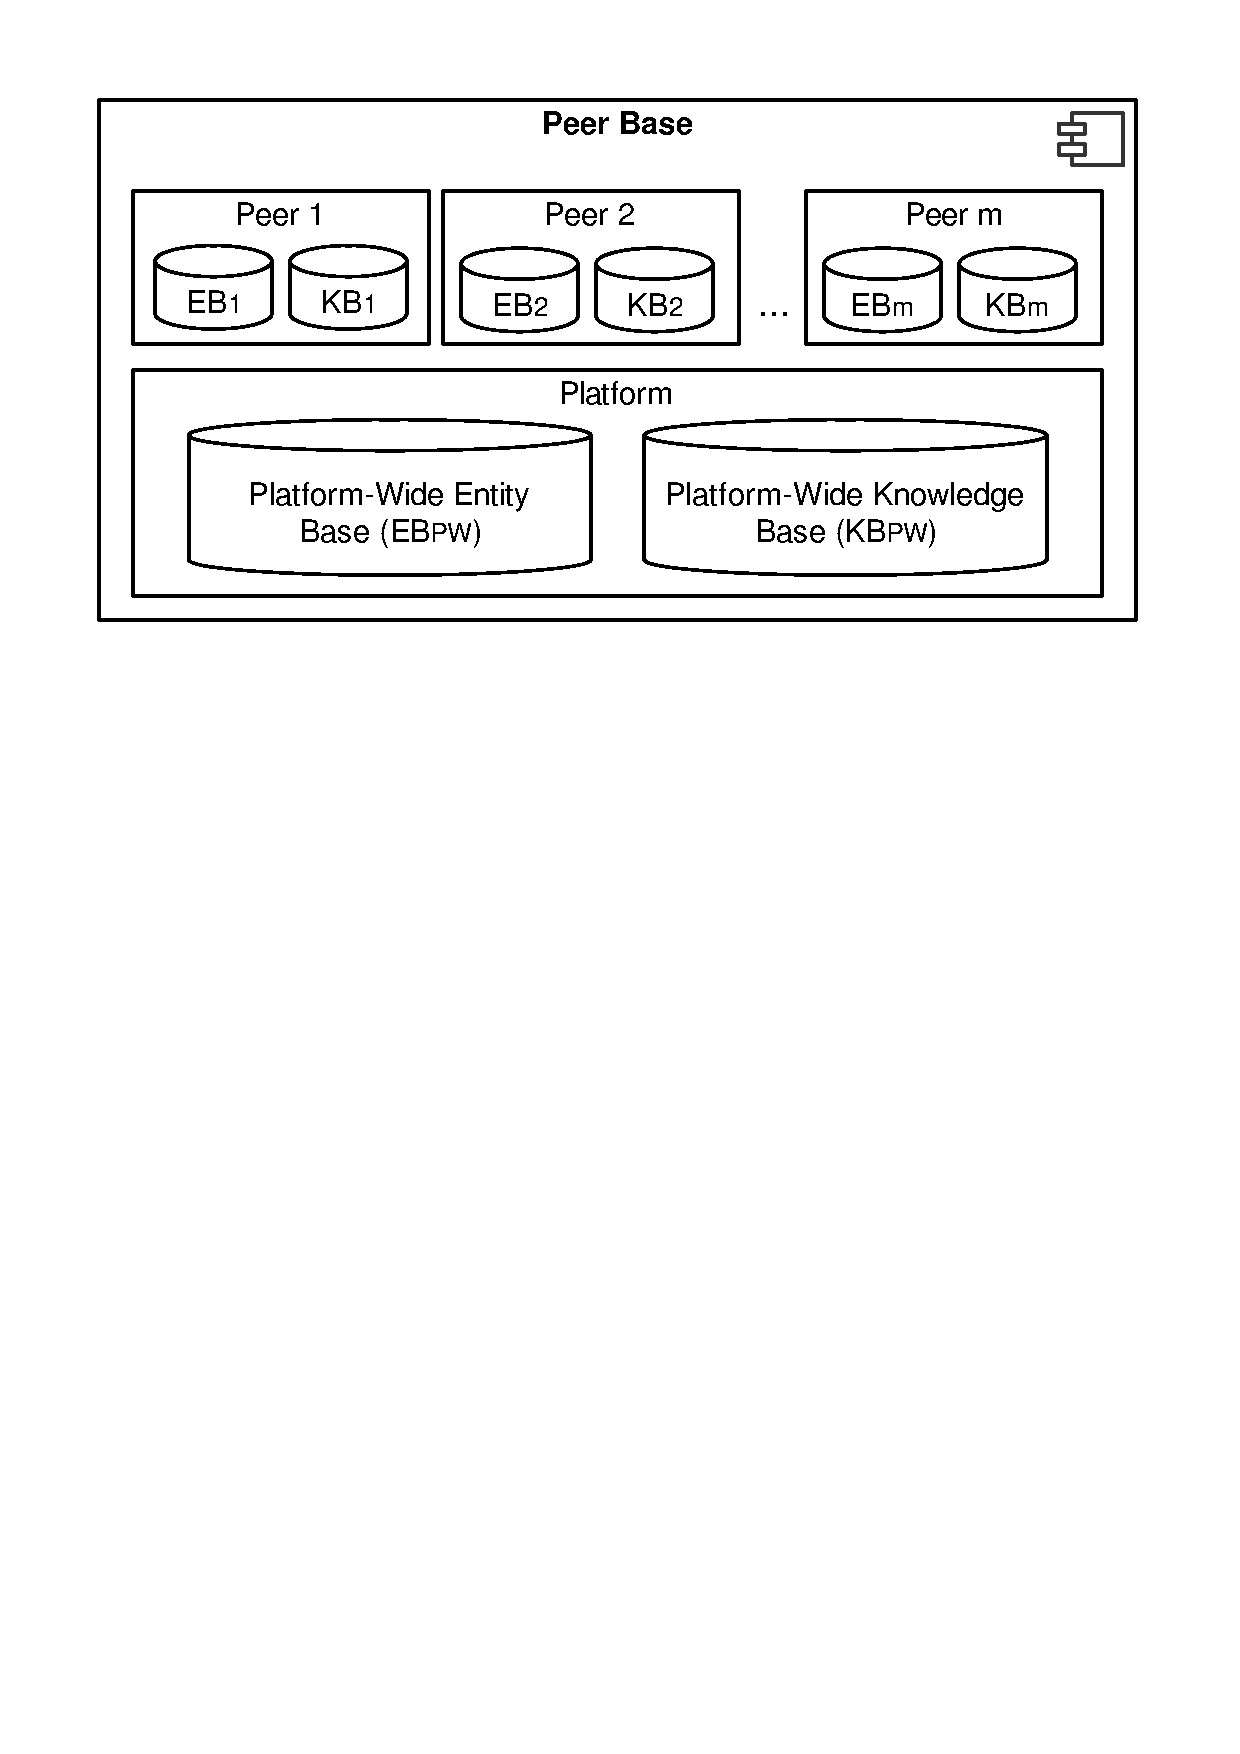
\includegraphics[width=0.65\linewidth]{figures/peerBase-diagram.pdf}
	\caption{Partial view of the Peer Manager internal architecture. Each subject its assigned its own peer storage, while the platform itself offers a shared Knowledge and Entity storages for different interactions.}
	\label{fig:peerManagerPlatform}
\end{figure}




\subsection{Implementation}
%{\it including how it has been implemented and specifications of APIs}

The Peer Manager component has been developed by following a three -layers approach, where each layer leverages the basic services offered by the level below and composes them for producing higher-level services. The resulting structure is shown in Figure~\ref{fig:pm-component-layers}; each layer will be further described in the remainder of this section. 

\begin{figure}[htbp]
\centering
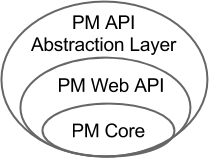
\includegraphics[width=0.3\textwidth]{figures/pm-component-layers.png}
\caption{Implementation layers of the Peer Manager}
\label{fig:pm-component-layers}
\end{figure}


\subsubsection{Peer Manager Core}
The Peer Manager Core provides a privacy-aware semantic storage for the SmartSociety Platform. This layer is implemented using Java, along with common data access frameworks like Spring and Hibernate.
While these technologies represent previous work from the University of Trento, the SmartSociety (through the work documented in~\cite{D1.1,D4.1,D4.2}) has created the Knowledge Model used for representing peers, users, profiles (i.e. personal information) and more generally managing the information for running an HDA-CAS.

No major changes have been done to the models or structures of the Peer Manager during the first half of Y-3 (so the research reported in previous deliverables still holds) but efforts to update these models to its final version will start in the second part of the year (as T1.4 restarts) and will have its results reported in Deliverable D1.3. No major changes are foreseen, so the underlying code and the exposed interfaces will likely be subject to minor revision only. 

\subsubsection{Peer Manager Web API} \label{ssec:pm-web-api}
This layer takes the Java classes that implement the Peer Manager Core and wraps them in HTTP API calls. 
No major changes to the APIs described in~\cite{D4.2} were introduced in Y-3. API specifications for this layer may be found in the Appendix~\ref{sec:pm-web-api-detail}.

\subsubsection{Peer Manager abstraction layer API} \label{ssec:pm-abs-api}
\todo{Content describing the purpose of this layer and the technologies used to implement it will be added to this section for the final version of this document}
 
This is a new component being developed specifically for the SmartSociety project and as such all code belonging to this layer will be open sourced. API Specifications for this layer may be found in the Appendix~\ref{sec:pm-abs-api-detail}.

\subsubsection{Integration Approach with PPL policy language}
\todo{Add A-PPL and Pii to the list of acronyms}

The Peer Manager theory presented in previous WP4 deliverables mentioned the need to include commonly agreed data handling policies between the source of the data (e.g. the person sharing the information) and the new data controller (e.g. the person that has received this information). Furthermore, one of the main novelties on the way that the Peer Manager handles this, is that the system will be able to enforce this commonly agreed data handling policy (named "agreed requirements" inside the Peer Manager theory) directly.

Previous iterations of the theory and architecture pointed that this would be done through integration of the Peer Manager and the PPL [?ref?] policy language but it is in this subsection where the first details and implementation details of such integration will be reported. 
In a close collaboration between the University of Trento and the University of Karlstad the following two approaches for integrating the PM (as defined in the year2 deliverable) and A-PPL engine (A-PPLE or A-PPL), which is Karlstad's current implementation of the PPL model, were defined:

\begin{enumerate}
	\item \emph{Basic integration approach}: the main idea of this approach is that both the PM and PPL run as different independent services within the same server and that they exchange information through their general web APIs. In practice (and as shown in Figure~\ref{fig:pm-ppl-lv1.png}) this will mean that the information in the Peer Manager profiles is not directly accessible (e.g. it is encrypted) and it is not readable without having access to the key being stored in a Pii (Personal Identifying Information) structure within the A-PPL system  (e.g. an encryption key). To authorize a request the A-PPL system will read the policy in the "agreed requirements" and evaluate the current request complies with them sending back only a "allow" or "deny" response to the PM. 
	\item \emph{Advanced integration approach}: in this approach both systems are still running independently in the same server but the PM does understands how to read and enforce the agreed requirements encoded in PPL. The policies are still being created and stored in the A-PPL system and are dereferenced (as shown in Figure~\ref{fig:pm-ppl-lv2.png}) by the use of their identifiers.
\end{enumerate}

\begin{figure*}[htb!]
\centering
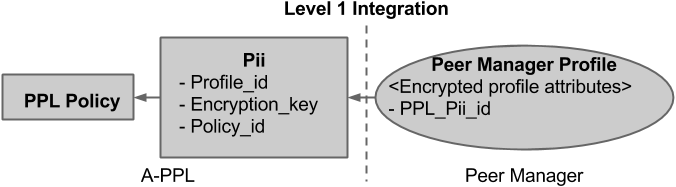
\includegraphics[width=0.8\linewidth]{figures/pm-ppl-lv1.png}
\caption{Basic Integration between the PM and PPL.}
\label{fig:pm-ppl-lv1.png}
\end{figure*}

Regarding the basic integration approach shown in Figure~\ref{fig:pm-ppl-lv1.png}, it is important to note that the actual attribute information in the profile is not immediately accessible even to its owner and to read this information it needs to read the corresponding Pii entity stored in A-PPL (thus having to comply with the policy that protects the Pii). This is the simplest way to achieve integration while being absolutely sure that A-PPL authorizes the reading of the information in the Peer Manager Profile. Nevertheless, it is only suitable for test research purposes for the following reasons:
\begin{itemize}
	\item Time and space overhead of having the two systems running and parallel without acknowledging their close interaction. Even though both systems are running in the same server, for large volumes of data and users this overhead is bound to become significant
	\item Security issues, having only a single unchanging encryption\_key for each profile undermines purpose biding as you could ask access to the info for one purpose and then there is no system-level check preventing you from using the info for other purposes.
\end{itemize}

Even with the previous issue the basic integration approach has still value for Proof-of-Concept integration and for small testing exercises. 

\begin{figure*}[htb!]
\centering
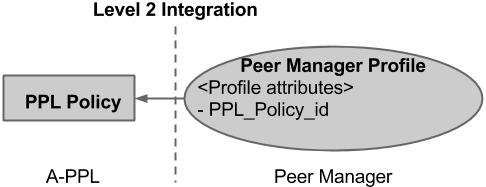
\includegraphics[width=0.6\linewidth]{figures/pm-ppl-lv2.png}
\caption{Advanced Integration between the PM and PPL.}
\label{fig:pm-ppl-lv2.png}
\end{figure*}

The mentioned problems are addressed within the advanced integration approach shown in Figure~\ref{fig:pm-ppl-lv2.png}. Here the A-PPL system is still used for the Policy storage and while the PM is supposed to have still no knowledge of how these policies are represented internally, the difference of this approach is that the PM does now understand how to enforce them. The Peer Manager will still ask the A-PPL system if a requested operation complies or not with a given policy, mainly because the PM does not share the same semantic ontology as A-PPL so it cannot know if a request complies with a Policy even if it has all information about both structures. This semantic heterogeneity is bridged by still keeping the two systems collaborating and running in the same server and while this does involve space and time overheads, they are of less importance than those of the previous approach (as the PPL already understand how PPL policies work but still needs to ask A-PPL to write and read these policies).

A third integration approach may be proposed at this point, involving the migration of the ontology that A-PPL uses for creating and interpreting the policies to the Peer Manager as a separate Knowledge Base (KB) belonging to a "A-PPL peer". Once this is done the Peer Manager will be able to support and enforce PPL without ever needing to call the A-PPL system, the A-PPL peer will then become a special privileged peer providing the service of writing and interpreting PPL policies within the SmartSociety platform. 

\subsubsection{Implementation of the Basic Integration Approach}
\todo{Data flow diagrams for the two example operations can be provided if deemed interesting}
\todo{Add appendix with A-PP call prototypes}
The current integration of the Peer Manager and PPL policies follows the 'basic' integration approach detailed in the previous section. This means that both A-PPL and the PM services are running independently in the same server and contacting each other via their HTTP APIs.

The implementation status of this integration is currently being tested and debugged to allow its use in future SmartSociety platform validation exercises. Specific details of the A-PPL calls being used by the PM for this integration can be found in the Appendix~XX and below we present two examples of the flow between the two systems.
\begin{itemize}
	\item \emph{Creation of a Profile}: when the PM receives a request to create a new profile, it makes the following steps:
	\begin{enumerate}
		\item The Peer Manager creates a profile: the PM creates the profile structure and users the information passed with the profile creation request for populating the information of that profile.
		\item The Peer Manager encrypts the profile information: the PM encrypts all the content information within the profile (do note that currently a dummy encryption algorithm is being used but this can be replaced when using in testing systems).
		\item The Peer Manager sends a CreatePII call to A-PPL: the PM uses the CretePII call to send A-PPL the encryption key that can be used to unencrypt the profile, along with the policy requirements sent to the PM in the request for creating the profile. Upon receiving this information A-PPL will create a new Pii structure that will use to contain the encryption key and will also create a new policy structure based on the policy requirements received from the PM that will restrict access to the previously created Pii.
		\item The Peer Manager stores the id of the created policy: the PM receives back an identifier of Pii created in A-PPL and stores it unencrypted in the source profile for future referencing.
	\end{enumerate}
	\item \emph{Reading of a Profile}: when a request for reading information inside of a profile arrives to the Peer Manager, it makes the following steps:
	\begin{enumerate}
		\item The Peer Manager sends a getPII call to A-PPL: using the identifier of the Pii stored unencrypted in the profile (last step of the previous example) along with the details of the purpose of the read request, the PM constructs a getPII call and sends it to A-PLL.
		\item The Peer Manager unencrypts the profile information: if A-PPL authorizes the previous request, it returns the encryption key to the PM and the profile information is unencrypted (otherwise a negative message is passed and the request fails).
		\item The Peer Manager answer the request with the requested data: the PM answers to the original request with the least amount of information necessary to address it.
	\end{enumerate}
\end{itemize}